\chapter[High Resolution Spectrometers (HRS)]{High Resolution Spectrometers (HRS)
\footnote{
  $CVS~revision~ $Id: hrs-1999.tex,v 1.7 2008/04/01 16:51:59 lerose Exp $ $ 
}
\footnote{Authors: J.LeRose \email{lerose@jlab.org}}
}
\label{chap:hrs}
\section{Overview}
   
The Hall A spectrometers and associated instrumentation are designed to 
perform high resolution and high accuracy experiments.  The goal is to 
achieve a missing mass resolution of $\sim$ 200-500 keV to clearly 
identify the nuclear final state.  An absolute accuracy of $\sim$ 1\% is 
also required by the physics program planned in the Hall, which implies 
$\sim$ 10$^{-4}$ accuracy in the determination of particle momenta and 
$\sim$ 0.1 mr in the knowledge of the scattering angle.

The instruments needed are a high resolution electron spectrometer 
(HRES) and a high resolution hadron spectrometer (HRHS), both with a 
maximum momentum capability matching the JLab beam energy, and large 
angular and momentum acceptance.

\begin{figure}[tbp]
\begin{center}
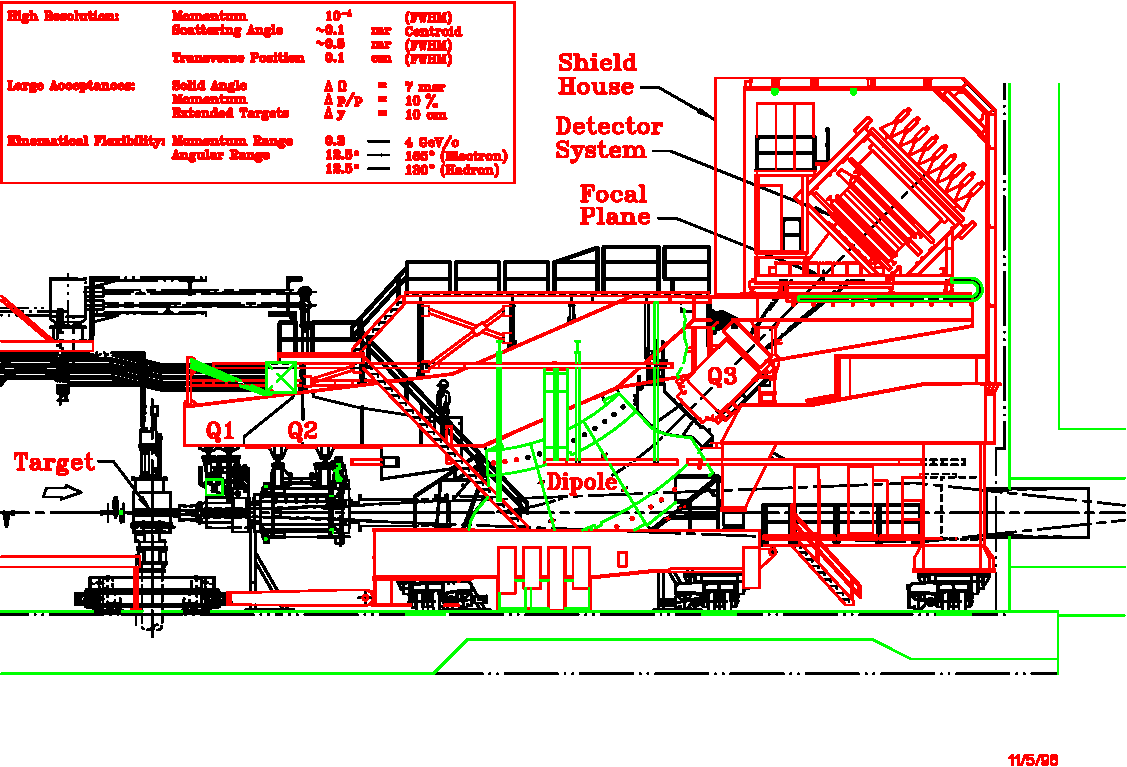
\includegraphics[angle=0,width=0.9\textwidth,clip]{figure0101_r}
\caption[Spectrometers: Elevation View of Hall~A HRS]{A side view of the Hall~A
HRS spectrometer.}  
\label{fig:hrs_ev}
\end{center}
\end{figure}
 
\begin{figure}[tbp]
\begin{center}
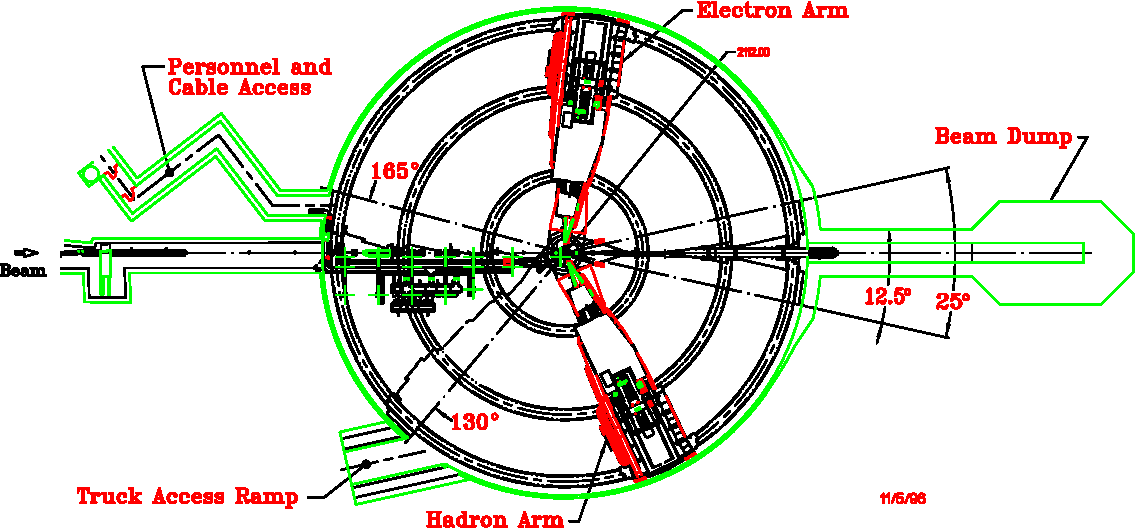
\includegraphics[angle=0,width=0.9\textwidth,clip]{figure0102_r}
\caption[Spectrometers: Plan View of Hall~A]{A bird's eye view of the Hall~A
end-station at TJNAF.}  
\label{fig:hrs_pv}
\end{center}
\end{figure}


A layout of the 4 GeV/c High Resolution Electron Spectrometer is shown 
on Figures~\ref{fig:hrs_pv} and \ref{fig:hrs_ev}.
Its main design characteristics are 
given in the attached table.  The spectrometer has a vertical bending 
plane and 45$^{\circ}$ bending angle.  The QQDQ design includes four 
independent superconducting magnets, three current-dominated 
cos2$\theta $ quadrupoles and one iron-dominated dipole with 
superconducting racetrack coils.  The second and third quadrupoles of 
each spectrometer have sufficiently similar field requirements that they 
are of identical design and construction.  The overall optical length, 
from target to focal plane, is 23.4 m.  Optically, the HRHS 
is essentially identical to HRES. In fact the two spectrometers can be used 
interchangeably to detect either positively or negatively charged particles 
as needed by any particular experiment. In fact, they are now commonly refered to 
as ``The Left Arm'' and ``The Right Arms'' rather than ``Hadron'' and ``Electron'' 

The support structure includes all system elements which bear the weight 
of the various spectrometer components and preserve their spatial 
relationship as required for 45$^{\circ}$ vertical bending optics.

The alignment and positioning system includes all the elements which 
measure and adjust the spatial relationship.  The support structure 
consists of the fabricated steel components which support the magnets, 
detector, shield house and associated equipment.  It is composed of the 
box beam, which supports the outer elements in fixed relative position 
atop the dipole; the dipole support bracket, upon which the dipole rests on 
the jacks; the cradle, upon which the dipole rests through the vertical 
positioning system, VPS; and a portion of the shield house load through 
the inboard legs of the gantry; the gantry, which supports the shield 
house and the magnet power supplies; and the bogies, which support the 
cradle-gantry assembly and slide on the floor plates and provide the 
driving power to move the two spectrometer arms.

The detector package (described in detail in Chapter \ref{chap:hrs-det})
is supported on the box beam and is surrounded by 
the shield house.  It must perform two functions, tracking and particle 
identification, PID.  The most important capability of focusing 
spectrometers is measuring precisely the momenta and entrance 
orientations of the tracks.  Momentum resolution of 10$^{-4}$ is 
obtainable, consistent with the resolution of the incident beam.

The actual configuration of the detector package varies from experiment to
experiment. The description given here is only an example of what is possible
and may well already be outmoded. 
\infolevone{
A particle traversing the detector stack 
(Figure~\ref{fig:hrs_electron_det}) encounters two sets of horizontal 
drift chambers (x,y) with two planes of 368
wires in each chamber. The track resolution is $\sim$ 100 $\mu$m.  
From the chamber information both 
positions and angles in the dispersive and transverse directions can be 
determined.  The information from these chambers is the principal input 
of the tracking algorithms.

The chambers are followed by a scintillator hodoscope plane designated S1. 
This plastic scintillator array provides the timing reference for 
the drift chambers, and is also used in trigger formation and in combination 
with a second hodoscope pair it can provide time of flight particle 
identification.  These scintillators can also be used to perform crude 
tracking.

The next element encountered by a particle is a gas threshold \Cherenkov{} 
detector.  This is used for particle identification.  In the hadron 
spectrometer this gas threshold \Cherenkov{} detector can be swapped 
against an Aerogel detector, with a similar function.

The second hodoscope plane, S2, is located directly behind the 
gas \Cherenkov{}.  Its function is essentially the same as that of S1.  
In the hadron spectrometer an option exists to have this hodoscope 
pair be preceded by a third chamber, to improve tracking.
 Each of the two spectrometers 
have gas and Aerogel \Cherenkov{} detectors which can be used
 when they are in electron detection mode.

The final elements in the detector stack on HRSE are 
the pre-shower and the lead glass shower 
calorimeter.  This is used for energy determination and PID.

\begin{figure}[tbp]
\begin{center}
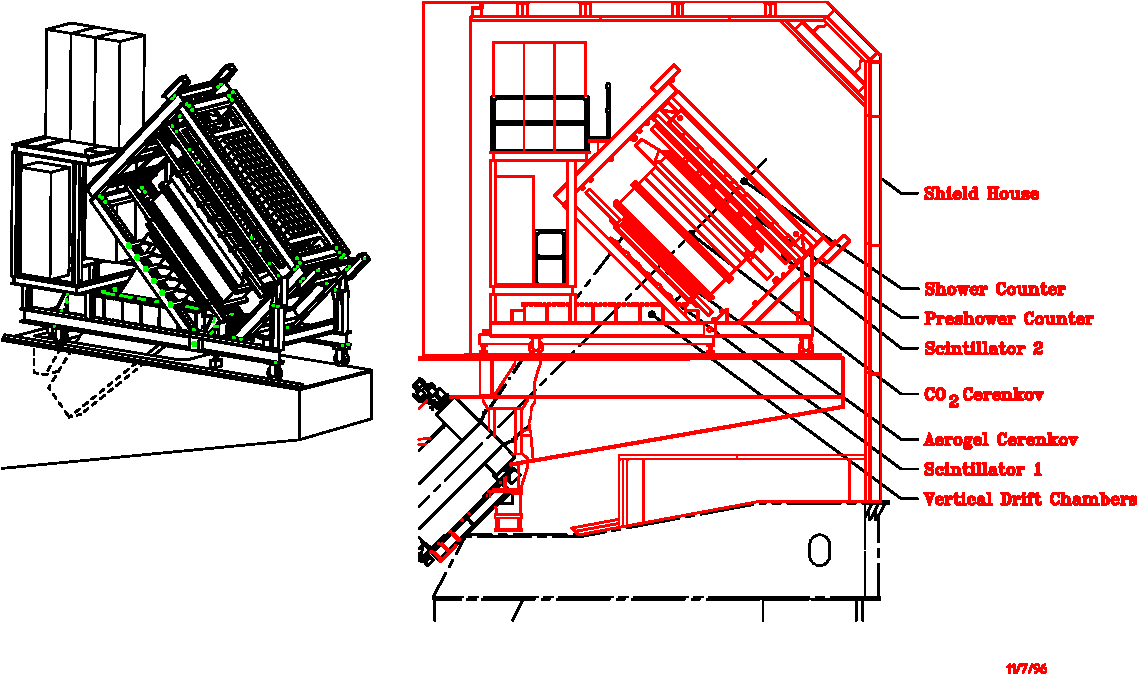
\includegraphics[angle=0,width=\textwidth,clip]{figure0103_r}
{\linespread{1.}
\caption[Spectrometers: Electron Arm Detectors]{The electron spectrometer detector stack.}
\label{fig:hrs_electron_det}}
\end{center}
\end{figure}

\begin{figure}[tbp]
\begin{center}
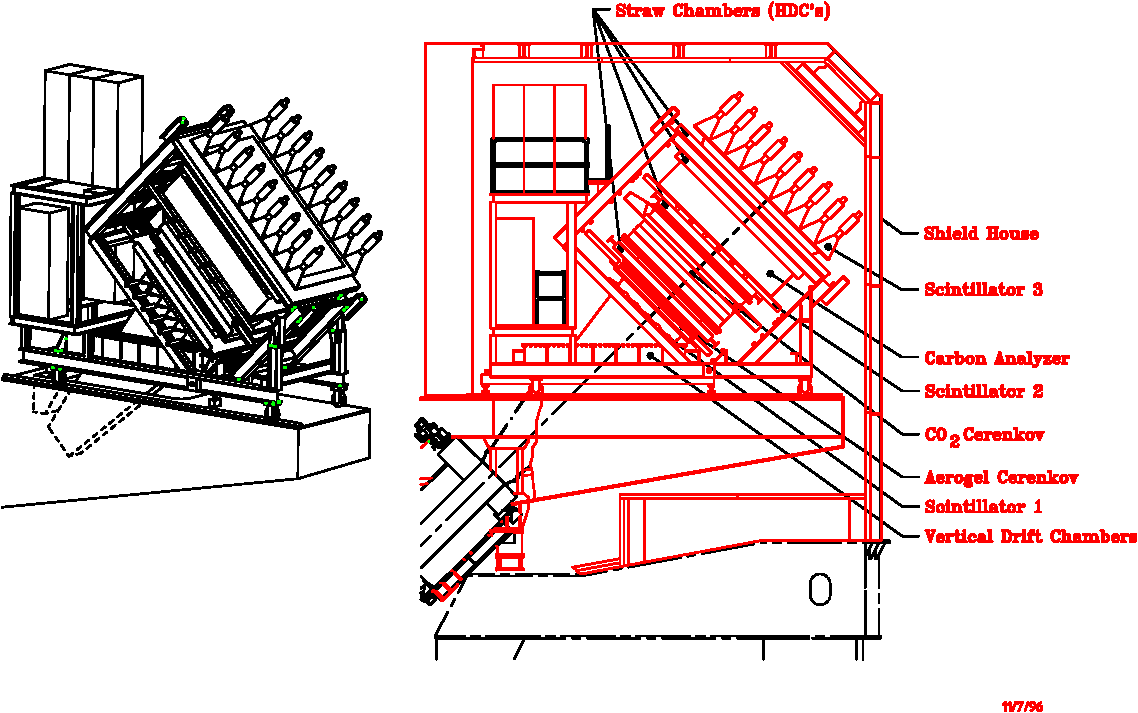
\includegraphics[angle=0,width=\textwidth,clip]{figure0104_r}
{\linespread{1.}
\caption[Spectrometers: Hadron Arm Detectors]{The hadron spectrometer detector stack.}
\label{fig:hrs_hadron_det}}
\end{center}
\end{figure}


The hadron detector is shown schematically in 
Figure~\ref{fig:hrs_hadron_det}.  It consists 
of two sets of (x,y) vertical drift chambers identical to those of the 
electron arm.  The remaining part of the detection system is used to 
define the level 1 trigger, as well as for particle identification and 
timing.  It consists of three minimally segmented planes of 
scintillation counters equipped with photomultipliers at both ends, and 
it includes \Cherenkov{} counters (gas CO$_2$ and Aerogel).

In addition, a proton polarimeter is installed in the back of the 
detector package to measure the polarization of the proton using a 
segmented carbon analyzer up to 60 cm in thickness to allow measurements 
over a wide range of proton energies.  A pair of front and a pair of 
rear straw chambers determine the incident and 
scattered angles, respectively.  The third scintillation counter, 
located at the rear end, provides the trigger for the polarimeter.  The 
polarimeter detectors are dimensioned to accept a 20$^{\circ}$ cone of 
scattered protons.

Several support systems are necessary in addition to the basic 
components mentioned above.  They include gas supply systems for the 
wire chambers, high voltage supplies, readout electronics, a second 
level trigger, software for data analysis and testing, and a remotely 
controllable mechanical system.

As for the electron spectrometer, all detectors are mounted on a 
single rigid carriage along with their associated electronics.  The FPP 
components are mounted on an FPP subframe for installation and removal as 
a unit.  The trigger electronics are located next to the detectors, 
as for the electron arm.

} %infolev

To reduce the resolution degrading effects of multiple scattering, the 
entire interior of the spectrometer from the pivot to the detector hut 
is a vacuum vessel.  The ends of this evacuated volume are capped by 
relatively thin vacuum windows.

\obsolete{
As mentioned, subsystems will be discussed in more detail in the next 
three sections.  The remainder of this section will describe some 
features common to the two spectrometers, then the following major 
sections will be devoted to the specifics that are not common.
} % obsolete

\begin{safetyen}{10}{15}
\section{Safety with Regards to the Spectrometer}
\label{sec:hrs-safety}
\end{safetyen}

The principle concern with the spectrometers is that they are large, 
and have associated vacuum, hydraulic, cryogenic and magnet systems all of 
which can be potentially dangerous.

The bogies which move the massive 1200 ton spectrometers must be 
carefully operated.  Inspection of the floor and wheels to ensure there is no 
debris which the wheels could ride over is mandatory.  Similarly 
personnel need to be aware that the spectrometers are moving so that no one 
inadvertently gets trapped.

The vacuum systems associated with the spectrometers are essentially 
pressure vessels (see Chapter \ref{chap:vacuum} for more details).
Care should be exercised so as not to puncture the 
windows.

The magnets themselves are installed inside cryostats.  These vessels 
are exposed to high pressures and are therefore equipped with safety 
relief valves and burst discs.

The hydraulic system that operates the vertical positioning system VPS 
and the horizontal positioning system HPS operates at high pressure, 
3000 - 5000 psi.  Therefore one should be careful when operating those 
systems.

The cryogenic system operates at elevated pressure at 4K.  One must 
guard against cold burns and take the normal precautions with pressure 
vessels when operating this system.  Only the JLab Cryogenics Group are permitted to install 
and take out U tubes.

The magnets have a great deal of stored energy as they are large 
inductors. Always make sure people are clear of them and that
the dump resistor is attached to the magnet.

There are several major safety concerns with regards to the detectors, 
namely 1) flammable gas located in the VDC and FPP, 2) ODH hazard due to 
CO$_2$ in the \Cherenkov{} counter, 3) high voltage due to the photo 
multipliers on the various detectors and 4) a thin vacuum window 
separating the detector array from the vacuum system in the 
spectrometers.  The clean agent fire suppression system, while installed 
to suppress fires, can also be a safety hazard.  It is possible for an 
individual to drop down alongside the box beam to the gantry roof 
inside the shield house.  This area, although technically not a confined 
space, could conceivably become one in the event that the clean agent 
system was activated.  Personnel should have a 5 minute air pack with 
them in the event they must enter the area alongside the box beam to the gantry roof 
inside the shield house.

\infolevltone{
\begin{safetyen}{5}{10}
For more information consult the full OSP manual~\cite{HallAosp}.
\end{safetyen}
} %infolev

\begin{safetyen}{10}{15}
\subsection{Authorized Personnel}
\end{safetyen}

In the event that problems arise during 
operation of the magnets, qualified personnel should be notified
(see Table \ref{tab:hrs:personnel}).  
This includes any prolonged or serious problem with the source of magnet 
cryogens (the ESR).  On weekends and after hours there will be a 
designated individual on call for magnet services.  Any member of the 
Hall A engineering group is qualified to deal with unusual magnet 
situations but in the event of serious problems the technician on
call should be contacted.

\begin{namestab}{tab:hrs:personnel}{HRS: authorized personnel}{%
      HRS: authorized personnel. ''W.B'' stands for the white board 
      in the counting house.}
   \TechonCall{\em Contact}
   \EdFolts{}
   \ScotSpiegel{}
   \MarkStevens{}
   \GaryDezern{}
   \ToddEwing{}
   \HeidiFansler{}
\end{namestab}


\infolevone{
\section{The Magnets of HRS}

Each HRS is composed of three superconducting quadrupole magnets, Q1, Q2, 
and Q3, and one superconducting dipole magnet.  The large quadrupoles were 
manufactured for JLab by SIEMENS, the small quadrupole by SACLAY, while 
the dipole was built for JLab by WANG NMR.  The quadrupole magnets are 
referred to as Q1, Q2, and Q3, where a particle first traverses Q1, then 
Q2 and the dipole magnet and finally traverses Q3. Also available as a separate
setup are a pair of superconducting warm bore septum magnets which provide
 angular coverage down to 6$^{\circ}$. 

The magnet system is followed by a large steel and concrete detector 
hut, in which all detector elements reside.  Most of the 
detector elements have been built by universities involved in the Hall A 
physics program.

The HRS magnet system is the cornerstone of the Hall A activities.  
Many of the experiments approved in Hall A center on physics at high 
resolution and other short-range phenomena, and rely on a spectrometer 
able to momentum analyze charged particles up to very high momenta.  The 
design value for the maximum momentum accessible to the HRS magnet 
system is 4 GeV/c.

\subsection{Magnets and Power Supplies}

The HRS magnet's are all superconducting and hence their coils must be 
maintained at cryogenic temperatures during operations.  The LHe 
required by the magnets is supplied by the End Station Refrigerator, ESR.

All the HRS magnets cryogenic services are supplied through the overhead 
cryogenic lines.  The distribution network begins at the distribution 
box over the pivot.  This box is connected to the rest of the network 
via the flexible transfer lines over the pivot.  The network is adjacent 
to the upstairs catwalk of the HRS.

Cryogenic information about each magnet is available on the control 
screens in the counting house, one for each magnet.  Normally during run 
periods the control screens are sent upstairs to the Hall A counting 
house and information on all the HRS magnets is available on the HRS 
control screen located in the center of the main console.  The control 
of all magnets is described in a following Section.

The power supplies for the magnets are located on the gantry balcony 
adjacent to the magnets.  The supplies are all cooled with LCW.

\begin{safetyen}{10}{15}

The front panels of the power supplies are interlocked.  Under no 
circumstances should the front panel of any supply be opened by anyone 
other than authorized personnel.  There is a keyed electrical interlock 
located in the Hall A counting house main console to prevent the power 
supplies from being energized at inappropriate times.  There are also 
signs posted listing the dangers of high magnetic fields.
\end{safetyen}

The control interface for the power supplies is available through the 
HRS control screen in the Hall A counting house.

\subsection{Quadrupole Magnets}

The quadrupoles provide some of the 
focusing properties of the spectrometer and to a large extent 
its acceptance.  Operating limits imposed on the 
quads are as follows: 1850A for Q2 and Q3 and 3250A 
for Q1.

All three quadrupoles for the HRS spectrometer are warm iron 
superconducting magnets.  The soft iron around the superconducting coil 
enhances the field at the coil center and reduces stray fields.  The 
basic parameters for the first quadrupole, Q1, are an effective length of about 
0.9 $m$, useful aperture of 0.3 $m$ and a field gradient of 9.5 
T/m.  To achieve the lowest possible angle setting of the HRS 
spectrometer (with respect to the beam line) the incident electron beam passes through
a notch in the outer yoke of Q1 when the spectrometer is at
its smallest angle of 12.5$^\circ$ . The 
other two quadrupoles Q2 and Q3, are essentially identical with an 
effective (magnetic) length of about 1.8 meter, a useful aperture of 
0.6 $m$ and a field gradient of 3.5 T/m.
} %infolev

\infolevthree{
The maximum operating currents (assuming a 4 GeV/c momentum particle) 
for the quadrupoles are about 3000 A, 1700 A, and 1600 A, for Q1, Q2, and 
Q3, respectively.  This will render pole field values 
of 1.2, 1.0, and 1.0 T, respectively.  The energy stored in the 
quadrupole fields is sufficient to cause an unrecoverable quench if all 
the energy stored is dumped into the magnets.  Therefore a quench 
protection circuit is incorporated.  However, a quench can only happen 
if the cryomagnets have a helium level below the coil 60\% during operation.

The operating current to the Q1 quadrupole coils is provided by Danfysik 
System 8000 power supplies, which can operate up to 3500 A current and 5 
V.  The power supplies will be cooled with a combined maximum 
water flow of 45 liters per minute.

In addition to the main quadrupole windings, all quadrupoles have 
multipole windings.  To further optimize focusing properties of the HRS 
magnet system, it was intended to operate including some of these multipole 
trim coils in order to reduce higher order aberrations.
The operating current for these multipole corrections is 
small, only (the multipole corrections are typically less than 2\% of 
the main quadrupole field), of order 50 A, and will be provided by 
thirty two Lakeshore power supplies.  These power supplies can operate up to 
100 A current and 30 V voltage. Since the sextupoles were inadvertently 
installed rotated 90 $^\circ$ from their correct
orientation, these trim coils are now considered useless 
and there are at present no plans to use them.

\subsection{Cryogenic Procedures}

All cryogenics control is handled by the JLab Cryogenics Group.  The cryo control coordinator 
can be reached at the CHL (x7405) or by calling the MCC.

\subsection{First Time Startup Check List.}  

See attached check lists for all quadrupole and dipole magnets
 (Tables~\ref{tab:dip_check}, \ref{tab:q1_check}, and \ref{tab:q23_check}).
} %infolev

\infolevone{
\subsection{Dipole Magnet}

The dipole, by virtue of its field index, provides both
dispersion and focusing.  The present operations envelope 
states that the supply for the electron dipole may not be
operated at a current above 1800 A (4.4 GeV/c). The supply for the hadron
dipole may not be operated above 1200 A (3.2 GeV/c). 

The dipole for the HRS spectrometer is a superconducting, cryostable 
magnet.  Its basic parameters are an effective length of about 6.6 $m$, a 
bend radius of 8.4 $m$, and a gap width of 25 $cm$.  It is configured to 
achieve a 45 degree bending angle for 4 GeV/c momentum particles at a 
central field excitation of 1.6 T.  For the HRS dipole to reach 1.6 T 
an operating current of about 1500 A is required.
} %infolev

\infolevthree{
The dipole has been designed to achieve cryostability up to a field of 2 
T, and this property has been extensively tested up to a field of 1.6 T. 
 The cryostable coils are equipped with an energy removal circuit to 
cover the possibility of an unrecoverable quench.  However, this can 
only happen if the helium level drops below the coil during operation.  
The current to the coils will be provided by a Dynapower System power 
supply, which can operate up to 2000 A and 10 V.  This 
power supply is located on the gantry beside the dipole, and will be 
cooled with a maximum water flow of 35 liters per minute.  The flow of 
the magnet cooling water will be regulated by flow meters installed on 
the floor of Hall A.  The total water flow needed to cool the 4 power 
supplies for the HRS magnet system (dipole and quadrupoles) amounts to 
80 liters per minute, with a supply pressure of cooling water for Hall A 
of 100 psi.
} %infolev

\infolevone{
\subsection{\bf Septum Magnets}

The Septum Superconducting Magnet System (SSMS)
can be divided into 5 interacting subsystems: the vacuum system, the 
liquid helium (LHe) and liquid nitrogen (LN2) cooling circuits, the power supply 
and associated cold and warm power buss, the magnetic coils itself, and the 
programmable logic controller (PLC) based control system.  These subsystems 
will be described separately below.

\subsection {\bf Septum Vacuum System}

The Septum Magnets have warm bore tubes and therefore the Septum Magnet 
insulating vacuum system is completely independent from all and any other 
vacuum systems. There are NO vacuum system interactions between the Septum 
Insulating Vacuum and any other adjacent vacuum system. The Septum warm 
bore tube is a rigid stainless steel conductor which is completely self 
supporting and can withstand a greater than a 1 Atmosphere pressure differential 
in any direction. When the Septa are configured for some 
experiments, the beam vacuum extends without interruption from the accelerator 
injector to the Hall A downstream beam diffuser and through the warm bore of 
each Septum through both HRS' to the Titanium exit windows. Valves located at 
the up-stream end of the target and the downstream end of the exit beam line 
allow the volume associated with the magnet, target, and both HRS Spectrometers 
to be isolated.  With these valves closed, the experimental apparatus can be 
isolated from the Accelerator Beam Line for maintenance , installation or 
dismounting. Other Septum Experimental configurations such as GDH have vacuum 
configurations identical to past Pol.He$^3$ target operations where the beam 
vacuum terminates upstream of the target chamber with a window. Some Septum 
experiments will feature a vacuum scattering chamber with spectrometer entrance 
windows.  


\subsection {\bf The Septum Beam Vacuum}


For experiments with vacuum extending from the target chamber to the HRS exit windows 
the volume under vacuum after the entrance beam line  valve can be estimated by 
adding up the following sub-volumes:
\noindent The main scattering chamber shell, of length 2 meters and inside diameter 
1 m, which contains either waterfall or cryo targets.  The volume of the scattering 
chamber ignoring the small targets inside is estimated to be 6.3 m$^3$.
\noindent The Septum magnet warm bore tubes.  The total volume of the 0.90 m long, 0.25 Meter 
high and 0.15 - 0.25 Meter tapered is 0.045 m$^3$ each.
\noindent The existing HRS volume of 15 m$^3$ each.
\noindent The exit beam line up to the exit beam diffuser.  The length of this volume is 22.5 m 
and the inside diameter is ~ 0.6 m resulting in a volume of 6.4 m$^3$.

The total Septum Beam volume is estimated to be 42.8 m$^3$.

Each HRS has a spectrometer exit window described previously.

The entrance Beam line valve is interlocked to the beam line pressure and has a fast 
close mechanism. The Beam line vacuum is a part of the Hall A FSD system. A beam line 
pressure that exceeds 1 x 10$^{-5}$ Torr will cause a fast beam shutdown and a closure 
of the entrance beam line valve. This system and the vacuum dynamics of this system 
are not changed by the fact that the spectrometers are now connected due to the fact 
that the small apertures near the scattering chamber limit propagation of fast pressure 
waves from one spectrometer to another. The Titanium windows have a pressure rating that 
far exceed what can be expected from any beam line failure. A Titanium window that is 
subjected to a pressure inversion will be counter yielded and must be replaced.


\subsection {\bf Septum Insulating Vacuum}


The magnet insulating vacuum volume (approx. 1 m$^3$) will be evacuated initially by a 
turbo pump and then sealed off(assuming no leaks).The Vacuum volume is protected by 
two vacuum relief devices that can limit internal pressure to below 1.5 ATM absolute 
in the event of an internal leak(See BWXT SMA-312-2008-1). A failure of the insulating 
vacuum cannot influence adjacent systems of vacuum spaces. A failure of the SIV will 
cause a magnet quench if the Septum is operating and condensation if the Septum is cold. 
The Septum has interlocks that protect the magnet in the event of a loss of vacuum. The 
first level interlock will cause a Septum slow discharge if the TC gauge reads between 
5 and 30 microns and a fast discharge if the TC gauge exceeds 30 Microns. The SSMS is 
protected form harm by internal systems during a loss of vacuum and there are no systems 
beneath the Septum Magnets  that can be adversely affected by condensation.

 SIV pressure (vacuum) is measured by a thermocouple gauge located on the cryoreservoir, 
by a cold-cathode gauge mounted on the cryoreservoir, and by a cold-cathode gauge mounted 
on the lower magnet cryostat. All three gauges are readout and logged by the control system.  
Under normal conditions, when the magnet is warm a vacuum in the low 10$^{-5}$ Torr range is 
expected.  When the magnet is cold, additional cryo-pumping and the elimination of most 
outgassing reduces the pressure to the low 10$^{-7}$ Torr range.

\subsection {\bf Septum Cryogenic Cooling Circuits}
Each septum is a dipole magnet consisting of a superconducting coil and cold iron yoke in 
a single cryostat.  The coils are cooled by LHe flowing in 10 parallel paths of 3/8 inch Nickel 
tubes, each of which are attached to the yoke by numerous Nickel straps. An LN2 shield  box 
completely surrounds the cold mass, which consists of the coils and cold iron yoke.  
The LN2 shield is cooled by 8 copper tubes, which are soldered to the outer surfaces.  
The warm bore shield tube is cooled by conduction from the outer surface through soldered copper 
support tabs. Cryogens are fed to both the LHe and LN2 circuits via manifolds at the bottom of 
the magnet from reservoirs located in the control dewar at the top of the magnet.  Plumbing on 
the top of the magnet makes the connection from the reservoirs to the manifolds.  A photo of the 
cooling tubes is shown in Figure \ref{fig:septum-cooling} and a schematic diagram of the LHe cooling circuit 
is provided in Figure \ref{fig:septumcryo}.
} %infolev

\infolevfour{
\begin{figure}[htp]
\begin{center}
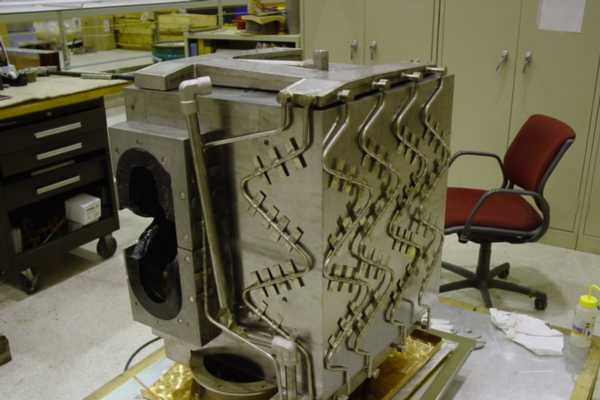
\includegraphics[angle=0,width=0.7\textwidth]{septum-cooling}
{\linespread{1.}
\caption[Septum: cooling channels on cold mass ]{Nickel Helium cooling tubes attached to the septum yoke}  
\label{fig:septum-cooling}}
\end{center}
\end{figure}
} %infolev

\infolevthree{
\begin{figure}[htp]
\begin{center}
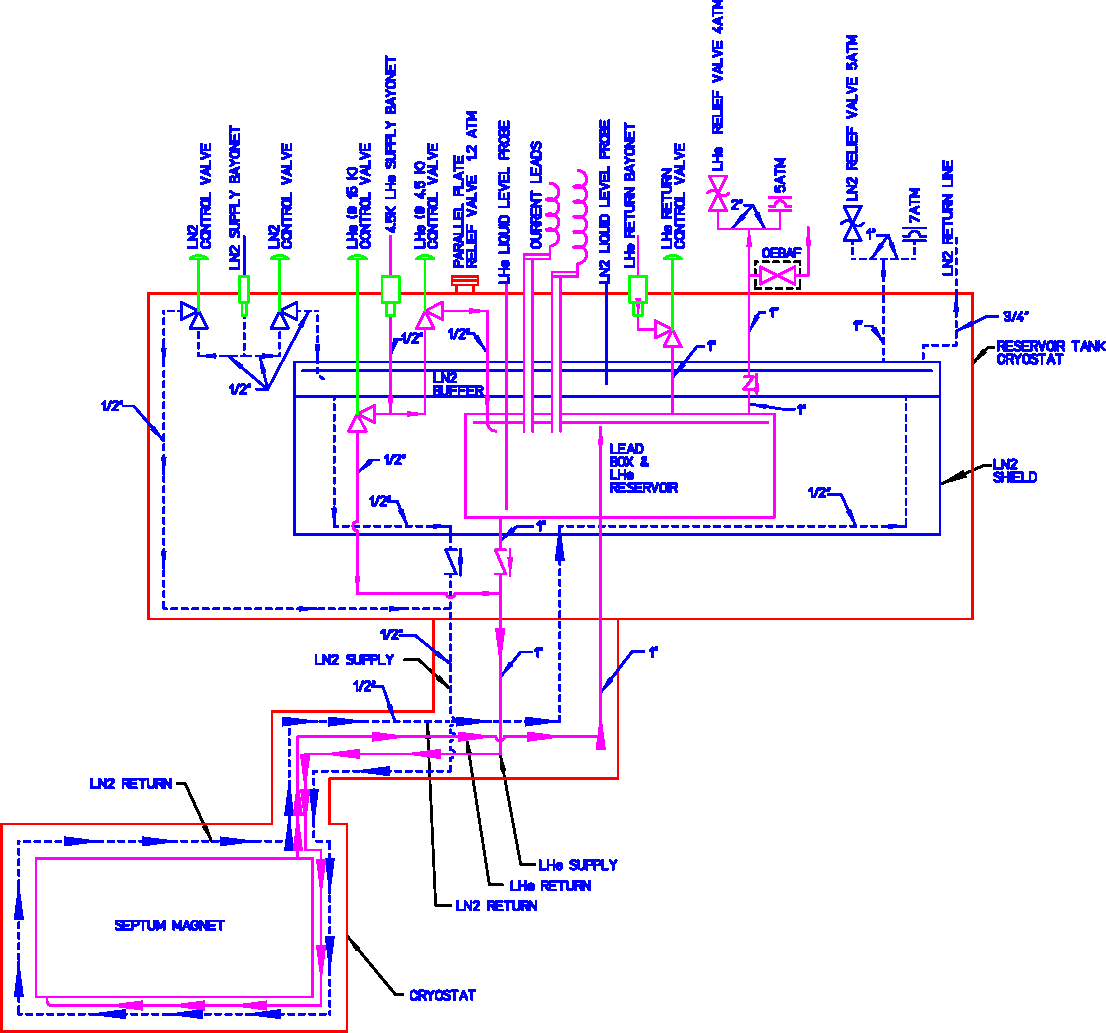
\includegraphics[angle=0,width=\textwidth]{septumcryo-diagram}
{\linespread{1.}
\caption[Septum: cryogenics diagram ]{Septum Magnet Cryogenic Diagramtum}  
\label{fig:septumcryo}}
\end{center}
\end{figure}


Normally, the magnet is cooled by thermal siphon flow.  Cryogens introduced at the bottom of the 
magnet from the reservoirs percolate back up to the reservoirs through the cooling circuit, losing 
density and absorbing power on the way.  Gaseous cryogens are exhausted and replaced by fresh 
liquid as determined by a control system PID loop which maintains the liquid levels in the reservoirs.

During cooldown, through the appropriate manipulation of cryogenic valves in the control dewar, it 
is possible to cool the magnet using forced flow.  In this mode, cryogens are introduced directly 
into the manifolds from the cryogen supply.  The connections between the cryogen supplies and the 
reservoirs are closed.  The reservoir drain valves, a manually operated plug valve in the case of 
the LHe circuit, and a check valve in the case of the LN2 circuit, are closed.  In forced-flow mode, 
cryogens returning to the reservoirs are not recycled through the magnet.  A detailed diagram of the 
cryogenic plumbing is shown in Figure \ref{fig:septumcryo} and a detailed Hall A flow diagram is available from 
the Hall A engineering group.

The temperature of the cold mass and LN2 shield is monitored by an array of thermal sensors, which 
are read by the control system.  Each coil is instrumented with two platinum resistance 
thermometers (PT-103) for the range from about 30 to 300 K and two CERNOX 1070 sensors for the 
range from 4 to 20 K and  four PT-103 sensors provide the temperature at various 
points on the surface of the LN2 shield.

The cryogen system can assume a number of useful configurations depending on the settings of the 
cryogenic valves.  These states are listed in Table~\ref{tab:septumcryo}.
 

\begin{table}[htp]
\begin{tabular}{|p{0.20\textwidth}|p{0.72\textwidth}|}
\hline
State        & Description \\ \hline
LN2 Cooldown & Begin forced-flow cooling of LN2 circuit.\\  \hline
Cooldown I   & Forced-flow cooling (or warm-up) of LHe circuit using 
               cas provided by CDHXR via JT-1. Inlet gas temperature 
               is regulated to be ~ 50 K below average coil temperature.
               Gas exhausted via warm return.\\  \hline
Cooldown II  & Cooldown of LHe supply line through reservoir fill (JT-2) 
               and exhaust through warm return. Plug valve closed.\\ \hline
Cooldown III & Cooldown of SSMS (plug valve opened) with gas from LHe supply 
               thru JT-1 and exhaust through warm return.\\ \hline
Cooldown IV  & Cooldown of cold return line by reverse flow through cold 
               return line (JT-3 open) and exhaust via reservoir through 
               warm return.\\ \hline
Run Mode     & Fill reservoir with LHe produced by JT cooling at JT-2.  
               Cool magnet in thermo-siphon mode.  Exhaust gas returned 
               through cold return.\\ \hline
Standby Mode & Magnet at LN2 temperature.  LN2 system in thermo-siphon mode. 
               LHe system cooled by 80 K helium from CDHXR in forced flow mode \\
\hline
\end{tabular}
\caption[Spectrometers: Septum cryo states]{Standard states of the septum cryogen system }
\label{tab:septumcryo}
\end{table}

In order to avoid thermal shock during especially in Cooldown I mode, the magnet temperature is reduced 
slowly from room temperature to about 100 K.  This is accomplished by introducing helium gas of variable 
temperature at a flow of about 10 g/s.  The gas temperature is adjusted by regulating the proportion of 
room temperature helium that is mixed with gas cooled by a LN2 heat exchanger (CDHXR).  The temperature 
of the gas supplied to the magnet is constrained by a control system PID loop to remain at no more than 
50 K below the average temperature of yoke and coils. This temperature is adjusted downward to maintain 
a 50 kelvin temperature differential between all parts of the cold mass.
} %infolev

\infolevone{
\subsection {\bf Septum Electrical Circuit}


A block diagram of the SSMS charging circuit is shown in Figure \ref{fig:septumcircuit}. Current is 
provided by a Power10 1000 A 
silicon-controlled-rectifier (SCR) based supply with an adjustable 10 V output.  It is a single quadrant 
power supply so slow ramp down is achieved through a bypass diode across the poser supply and the warm DC 
bus series resistance which provides ~ 2 volts. This feature is used to provide a ``slow-dump" function 
whereby the magnet current cab be zeroed with a time constant of 350 seconds. A ``fast-dump" capability 
is provided by a high-speed circuit breaker (manufactured by Scheron SA and rated at 1000 A and 1 kVDC) 
and an air-cooled high power resistor. (a Post-Glover resistor rated at 140 volts at 700 A with a 
resistance of 0.2 W). Quench detection, as well as a number of safety-related conditions will result in 
the initiation of a fast dump. In that event, the fast dump switch which is a normally open type looses 
its holding current and  opens to disconnect the power supply from the magnet. The stored energy of the 
magnet, 0.22 MJ at full excitation, is then dissipated by the dump resister with a decay time of 5 s.  
A shunt  is employed to measure the current supplied to the magnet and to provide feedback to the power 
supply for current regulation. The shunt would normally be housed within the power supply enclosure and 
measured the total output current of the supply.  With the dump resistor and magnet wired in parallel 
the precise measurement and regulation of the magnet portion of the current required that the shunt be 
relocated to a point in the circuit after the dump switch and dump resister.

\begin{figure}[tbp]
\begin{center}
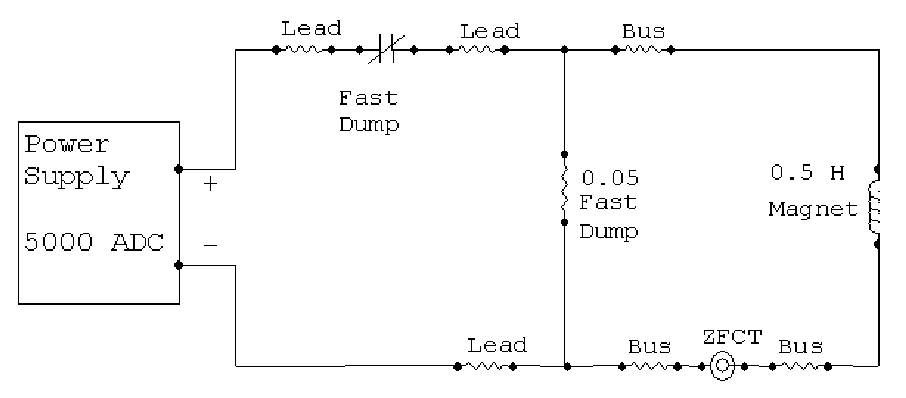
\includegraphics[angle=0,width=0.9\textwidth,clip]{septum-circuit}
{\linespread{1.}
\caption[Septum: circuit ]{Septum Magnet Charging Circuit}  
\label{fig:septumcircuit}}
\end{center}
\end{figure}
} %infolev

\infolevthree{
All interconnections between room-temperature components of the circuit are made with 1000 MCM flexible 
air cooled 
cable.  Power connections to the superconducting buss are made via vapor cooled leads (VCLs).  
These are designed to tolerate a 900 s slow dump after a complete interruption of coolant flow. 
Each lead consumes 1.8 l/hr/kA of LHe.  The flow of coolant gas is regulated and measured by flow 
controllers interfaced to the control system.

Each coil consists of a pair of 650 turn coils of superconductor wet wound in epoxy. Two voltage taps on 
the coil leads provide a measure of the coil voltage for the quench-detection systems.  In addition, 
voltage taps are located on the incoming ``transition leads" on the cold side of the VCLs within the 
LHe reservoir. Each voltage tap is isolated by a 10 kW (Cold value) resistor mounted on the coil.

Quench detection is provided by two parallel systems, a digital PLC-based system and a hard-wired 
analog system.  Both systems are designed to be insensitive to inductive voltages produced during 
ramping and to provide detection of quenches, not only in the coils, but in the transition leads.  
The analog quench protection system is considered a ``backup" for the digital system.  As such, its 
threshold is set higher.

The digital quench detection system employs isolation amplifiers each connected through a resistive 
divider to the voltage taps on the leads of a coil. Dividers are used to reduce each voltage tap signal, 
expected to reach 150 V during a quench, in order to protect the signal conditioners. The amplifier 
outputs, proportional to the coil voltages,  are fed to analog inputs of the PLC.  The PLC compares each 
coil voltage to the average for all eight coils.  If the deviation is greater than a set threshold, 
typically around 1 V, the quench protection system is triggered to generate a fast dump.  In addition, 
a series of thresholds are defined for the transition lead voltages, and a fast dump is triggered when 
the highest is exceeded.

The analog system follows a design developed in Hall A for the HRS magnets.  A simple threshold plus 
and minus voltage comparator is used to generate an analogue interlock. Exceeding the preset level 
generates a fast discharge.  A trace wire in each voltage sense cable provides an analogue interlock 
that insures that the cable is plugged into the magnet.
A second pair of discriminator channels are devoted to quench detection in the  vapor cooled leads.   
} %infolev


\infolevone{
\subsection {\bf Septum Control System}

The control system consists of three principle subsystems: 1) signal processing electronics, 2) the PLC 
and its ``ladder logic" software, and 3) the console (user interface) PC and the software that runs on it.  
The control system occupies three racks located behind the shielding wall in Hall A.
} %infolev

\infolevthree{
The signal processing electronics, provides conditioned (level shifted, gain adjusted, isolated, etc.) 
signals from sensors associated with other subsystems of the SSMS to the analog and digital inputs of the 
PLC and, in the exceptional case of resistance thermometers, to the console PC.  It also provides the 
necessary conditioning to interface analog and digital outputs from the PLC to actuators and external 
controls.  For the most part, the signal processing electronics is packaged in modular DIN-rail-mounted 
components.

A PLC is a special-purpose microprocessor optimized for process control applications.  The SSMS control 
system uses a Direct Logic DL405 PLC manufactured by Automation Direct.  Modules provided by the 
manufacturer for digital and analog input/output are used to interface to the outside world.  The PLC 
is programmed using relay ladder logic, a language that is not unlike assembly language of conventional 
microprocessors.  The ladder logic program is executed in a loop over and over again.  The minimum 
response time of the PLC is therefore the loop time, which for the SSMS control system, is about 25 ms.  
The analog inputs of the PLC are multiplexed so that eight analog inputs are read by a single ADC.  A 
single input for such a multiplexed ADC is read on each cycle through the ladder logic program.  
Multiplexing therefore further increases the PLC response time to analog inputs by a factor of 8 to 
about 200 ms. The PLC interfaces via the signal processing electronics to devices which measure cryogen 
pressure; cryogen reservoir level; LCW temperature, pressure, and flow; VCL gas flow; strain in warm-to-cold 
supports; coil and transition lead voltages; power supply parameters; cryogenic valve posi-tion; and vacuum. 
The PLC can set the cryogenic valve position, the VCL gas flow, the power supply current and on/off status, 
the dump switch position, and the cold-cathode vacuum gauge on/off status. The PLC also serves as a 
repository for information from the console PC.  This includes temperatures from resistance thermometers 
provided by the console PC temperature monitoring process and user-set parameters provided by through the 
user-interface program.  With these capabilities, the PLC provides the following functions:

\begin{list}{--}{\setlength{\itemsep}{0.cm}}
\item Analog inputs are scaled to ``engineering units" and stored as IEEE floating point num-bers.

\item Scaled analog values are compared to user-set levels and alarm indicators are latched when a level is passed.

\item Based on alarm indicators and digital inputs, interlocks are set which may initiate a fast or slow dump.

\item Cryogenic valve (JT valve) actuators are adjusted according to user-set target positions.

\item The power supply current is adjusted based on a user-set current and ramp rate.

\item Gas flow through the VCLs is adjusted based on user set values or automatically based on current.

\item Cryogen level and cooldown (or warm-up) is controlled using PID loops.
\end{list}

The third component of the control system is the console PC.  This Windows 2000 PC has three main functions.

\begin{list}{--}{\setlength{\itemsep}{0.cm}}
\item First, it serves as a development station for the ladder logic program running on the PLC.  A powerful 
graphical programming and debugging system (DirectSoft 32) allows one to create and document the PLC program, 
store it on local disk, download or upload it from the PLC via Ethernet and run it on the PLC.  There is no 
direct programming interface to the PLC; all programming is carried out through the console PC.

\item Second, the console PC also runs a dialect of the National Instruments human-machine-interface program 
called LookoutDirect.  Using screens created with LookoutDirect, one can monitor the status of analog digital 
signals, alter user-setable parameters in the PLC, command the PLC to perform control procedures and display 
the logged history of PLC acquired data.  Screens are for the following specific areas of the SSMS: alarm 
control, CDHXR, interlocks, JT valve control, VCL control, LHe level, LN2 level, LHe and LN2 cryogen circuit 
status, power supply control, quench protection, setpoints and levels, strain monitoring, temperatures, vacuum, 
and LCW monitoring.  Logged data is stored in compressed form by LookoutDirect and is available to any 
Microsoft Open Database Connectivity (ODBC) compatible application (including Excel) via the Citadel ODBC driver.

\item Third, resistance thermometers used to measure cryogenic temperatures are interfaced to the control 
system using eight-input temperature controllers manufactured by Lakeshore.  Those de-vices provide 
temperatures to the control system through a serial interface.  Six such con-trollers are used to allow 
48 temperatures to be read out.  There is not a convenient method to connect and read the serial outputs 
of the temperature controllers directly at the PLC.  In-stead, the Lakeshore controllers are initialized 
and read-out by a process on the console PC, which simply transfers temperatures from serial inputs on 
the PC to PLC memory via Ethernet.
\end{list}
} %infolev

\infolevone{
\begin{safetyen}{10}{15}
\subsection {\bf Septum Hazard Analysis and Control}
\end{safetyen}


Personnel and equipment safety hazards are associated with the operation of the SSMS.  
Without hazard controls, accidents involving serious injury, costly property damage, and loss of 
time are likely to occur.  However, if engineering and administrative hazard controls are implemented, 
the probability and consequences of accidents can be reduced the level of accept-able if not negligable risk.

In general, all who are involved in the operation of the SSMS must have completed all certification 
and training required for work in Hall A (Radition Worker, ODH, and EH\&S training and the Hall A 
walk-through), must be familiar with the current Experimental Safety Assessment Document (ESAD), 
if one is in place, and must have signed the Conduct of Operations (COO) appropriate to the current 
state of Hall A.  

In the following sections, the hazards associated with each of the SSMS subsystems are discussed.  The 
likelihood and the consequences of each hazard are assigned according to the criteria in Thomas Jefferson 
National Accelerator Facility Environment, Health, and Safety Manual[EHS] Section 3210.  
Controls for mitigating the hazard and their effect on the risk is estimated.


\begin{safetyen}{10}{15}
\subsection {\bf Septum Vacuum System Hazards}
\end{safetyen}


The principle hazard associated with the evacuation of the SEPTUM beam vacuum arises from the possible 
failure or damage to the target cell should the magnet beam vacuum be released while the cell is evacuated. 
This has consequence only if the septum magnets are vacuum coupled to the scattering chamber. This is 
assumed for this section. 

{\bf Target Cell Implosion Hazard:}
The first step in operating the target is the removal of all air from the target, ballast tank and
associated plumbing. To do this, the entire system is repeatedly evacuated and back-filled with pure 
gas. The first back-fill of any part of the system is with helium to reduce the possibility of mixing 
air and hydrogen. Subsequent back-fills of the target loop or ballast tank use hydrogen. The full 
procedures for purging the ballast tank and target cell are described in the Hall A Target User's section. 
It is imperative that the SSMS beam vacuum and target scattering chamber be evacuated before pumping on 
the target loop. The target cell is very thin and will implode if the pressure outside it exceeds the 
pressure inside.

Without controls, the likelihood of this occurrence is estimated to be ``likely to happen'' given 
sufficient time. (Likelihood Code C).  While there is no danger of personnel injury (the target is 
completely enclosed by the scattering chamber), the property loss, not to mention the labor required 
to replace the cell, would involve costs in the \$500 to \$10,000 range resulting in a Consequence 
Level of II.  The Risk Code with no controls is then 2.  In order to mitigate this risk, two controls 
are implemented: 
\begin{list}{\arabic{enumi}.~}{\usecounter{enumi}\setlength{\itemsep}{-0.15cm}}
   \item The engineering control of interlocking target pneumatic valve PV21 with vacuum 
       as indicated by the SSMS  beam vacuum cold cathode gauge to prevent pumping on the target loop unless 
       the vessel is evacuated.  If the gauge is turned off, preventing a valid vacuum measurement, the 
       interlock is opened and evacuation of the cell prevented.
   \item As a further control, any venting of 
       the SEPTUM beam vacuum must be approved in writing (or by e-mail) by the target person on-call.  
       With these controls in place, the likelihood of target cell implosion is greatly reduced.  The Risk 
       Code is mitigated to level 0.
\end{list}

\begin{safetyen}{10}{15}
\subsection {\bf Hazards Associated with the Cryogenic Cooling Circuits in Septum Magnets}
\end{safetyen}

In addition to the normal hazards inherent to cryogenic materials (e.g. the dangers of ``burns" and 
oxygen concentration near cold surfaces) the following hazards associated with the cryogens in the 
magnet plumbing have been identified.

{\bf Over-pressurization of cryogen plumbing:}  The most likely cause of this event is a sudden 
loss of the insulating vacuum (LOV).  This scenario was analyzed by the magnet vendor [BWXT SMA -312-2008-1].  
The analysis was done without consideration of the mechani-cal relief or the normal exhaust lines and 
therefore represents a worst case.  For the helium circuit, the report concludes that the helium pressure 
would not exceed 5 atm (the burst disk pressure) in the reservoir.  For the nitrogen system, the pressure 
will not exceed the burst disk pressure in either the reservoir or the piping.  The reservoirs and piping 
are quite capable of withstanding these pressures according to the design analysis performed by the magnet vendor.

While the calculations suggest that the system is theoretically safe, one can imagine conditions under 
which the assumptions of the analysis would be violated.  For example, faulty pipe material or a poor 
weld might be weaker than the design strength; or the relief path might become blocked by foreign or 
frozen material.  In such cases, the piping or joints might fail.

If the failure is internal to the cryostat, this could result in a large internal leak into the insulating 
vacuum, which might cause over-pressurization of the vacuum vessel.  The likelihood of a rupture in the 
plumbing during normal operation is estimated in Table \ref{tab:septumfail}.

\begin{table}[htp]
\begin{tabular}{|l|l|l|l|}
\hline
Equipment   & IndividualFailure Rate (/hr) & \# of Items & Total Failure Rate (/hr) \\ \hline
Pipes       & 1x10$^{-9}$                  & 35          & 3.5x10$^{-8}$\\
Valves      & 1x10$^{-8}$                  & 3           & 3.0x10$^{-8}$\\
Welds       & 3x10$^{-9}$                  & 35          & 1.1x10$^{-7}$\\ \hline
Total       &                              &             & 1.7x10$^{-7}$ \\ \hline
\end{tabular}
\caption[Septum: failures]{Septum failure rate estimates for internal plumbing }
\label{tab:septumfail}
\end{table}
	


For the purposes of this estimate, the number of welds and pipes was augmented by 20% and values for vacuum 
valves were assumed for the cryogenic valves.  The failuwre rate, driven by the possible failure of welds, 
implies one failure per 672 years, i.e. Likelihood Code A (very unlikely to occur) [EHS section 3210].  The consequences 
and risks of this hazard will be discussed fur-ther in item b below.  It is important to note that these 
estimates assume ``normal operation".  Inadvertent sudden cooling of the magnet could produce thermal 
contraction and shock, which would increase the likelihood of failure.  This possibility will be discussed 
later.

Another possibility is that faulty external plumbing might suddenly give way releasing cold cryogens and 
possibly ejecting fragments at high speed.  The relief of a burst disk entails similar consequences.  
Property loss would be minimal but personnel injury could be severe, though unlikely to be fatal.  A 
Consequence Level of III is therefore assigned to this type of event.  There are fewer pipes, valves 
and welds that are externally exposed, so external plumbing rupture can also be considered to be very 
unlikely to occur (Likelihood Code A).  However, a burst disk rupture is expected to happen given 
sufficient time (Likelihood Code C).  The greatest risk, a Risk code of 3, then comes from the possibility 
of injury due to burst disk fragments.

The risk can be reduced through the following controls:
\begin{list}{\arabic{enumi}.~}{\usecounter{enumi}\setlength{\itemsep}{-0.15cm}}
   \item Burst disks must be located at a height and orientation such that all fragments 
         are blown upward above anyone working in the vicinity.
   \item Where it is impossible to relocate the burst disk, a protective screen or tube must be installed.
   \item Warning signs must be installed near the burst disks.  These should tell workers 
         to avoid the immediate vicinity of the burst disks exhaust.
   \item Personnel working on the SSMS platform, near the burst disks and other 
         external plumbing, must be limited during cooldown to those who are aware of the hazard.
   \item Burst disks should be inspected regularly to ensure that no foreign material can block 
         their operation. Assuming that these controls are followed, the risk of personal injury 
         will be greatly reduced.  This will result in a reduced Risk Code of 1.
\end{list}


{\bf Over-pressurization of the vacuum vessel caused by leak in cryogen plumbing:} The likelihood 
of this event is estimated in Table \ref{tab:septumfail} to be very unlikely to occur (i.e. Likelihood Code A).  The 
consequences depend on whether gas leaking into the vacuum vessel can be adequately relieved.  The 
main vessel will withstand an internal pressure of 22 psia according to analysis by the vendor. The 
target service module was designed to withstand an internal pressure of 29.4 psia.  The vessel was 
successfully tested at UIUC, with all relief valves sealed, to a pres-sure of 2.21 psig as specified by 
the ASME code.  A titanium exit window was individually tested to a pressure of 165 psig.

There are 3 relief ports on the vacuum volume located: on the target service module, directly on the main 
cryostat volume (at the 315$^\circ$ position) and on the cryoreservoir.  K. Gustafsson has shown 
 that the relief valve on the target service module, alone, is sufficient to vent a leak of 2.5 atm 
helium at 4.5 K and 5 g/s flow.  The remaining relief ports are therefore sufficient to relieve the 
highest flow expected (during Cooldown I ) of 10 g/s, even if one becomes stuck or plugged with debris.  
The most serious consequence of this event is associated with the cost of repair of a major internal leak 
in the cryogenic system which is likely to be in the \$10k to \$100k range.  A Consequence Level of III is 
therefore assigned, resulting in a Risk Code of 1.

\begin{safetyen}{10}{15}
\subsection {\bf Hazards Associated with the Septum Electrical Circuit}
\end{safetyen}

The charging circuit for the SSMS provides, at full power, 700 A at about 10.0  V to the 1.0  H inductive 
load of the magnet and leads.  At full power the SSMS stores 0.22 MJ of energy.  The 2 volt drop, due to 
resistive losses in the air cooled leads implies a power dissipation of 1.4 kW.  The hazards associated 
with the electrical circuit arise from this large stored energy and power dissipation.

\begin{safetyen}{10}{15}
\subsection {\bf Septum Magnet Quench Hazard}
\end{safetyen}
If, for some reason such as local heating due to a heat leak or mechanical energy release, the superconductor 
in the SSMS becomes locally normally conductive (a quench), resistive heating will cause the normal zone of 
the conductor to propagate through the superconductor in 0.15 seconds! The Septum magnets are self protecting 
and the final coil temperature is ~ 120 Kelvin. The coils quickly come to equilibrium with the yoke at an 
estimated temperature of ~ 10 Kelvin overall. There are no cases where quench protection can remove any energy 
from the coil during a quench so magnet safety is not enhanced by quench protection. Quench protection can only 
protect the vapor cooled current leads from burn out in the event that lead coolant is lost . The maximum amount 
of stored energy that can be removed in a fast discharge with no initial quench is only 40\% due to self 
quenching upon fast discharge.

The method for detecting a quench is to sense the relatively large resistive 
voltage drop which accompanies local heating of the conductor.  This is accomplished by two parallel and 
independent quench detection systems.  The voltage threshold at which the quench is signaled is critical.  
Calculations indicate that  the stored energy cannot be dumped during a quench and that the final temperature 
is only 120 Kelvin. Redundancy is not required in the quench protection system because the coils are self 
protecting and the current leads are a no burnout design within the circuit decay tine of 350 sec-onds.


\begin{safetyen}{10}{15}
\subsection {\bf Hazards from Exposed High-current Contacts in the Septum Magnets}
\end{safetyen}

If metal tools accidentally come into contact with exposed leads on the SSMS or the power supply and short 
them out, the likely outcome will be vaporization of the metal tool and an arc flash which could cause 
severe burns.  When a quench is possible, even when the quench detection system is operating correctly, 
terminal voltages can exceed 50 V and there are significant (greater than 0.5 joules), conditions which 
can result in 
electrocution [EHSc].  With no hazard controls, an event of this kind is likely to happen (Likelihood Code C).  
Because death could result, the Consequence Level is IV and therefore the Risk Code is 5

Two controls are used to reduce the likelihood and severity of this hazard.  First, the power supply is equipped 
with a ground-fault detector.  Any current which leaves the power supply must return.  A short from a lead to 
ground results in the ground fault interlock being opened which leads to a fast-dump and power-supply shut-down.  
The second control is administrative in nature.  The areas inside and on top of the supply where there are exposed 
high-current leads will be protected by a barrier, which prevents any contact.  The power supply will be locked in 
the off state whenever the magnet platform must be accessed.  When the power supply is operated and connected to 
the magnet, no personnel will be permitted on the magnet platform. JLab rules also require that there be a red 
beacon to indicate that the SSMS is powered.  These controls reduce the Risk Code to 1 by making the probability 
of an electrical accident ``very unlikely to occur" (Likelihood Code A).

\begin{safetyen}{10}{15}
\subsection {\bf Hazards of Static Magnetic Field from the Septum Magnets}
\end{safetyen}

Because the septum magnets have a dipole field configuration with an iron yoke, magnetic fields external to the 
cryostat are not large. These fields are 50 - 100 gauss 
at ~2 feet from the septum magnet. Potentially fatal medical outcomes may result from exposure to magnetic 
fields in people who have ferromagnetic objects in their bodies.  A magnetic flux density exceeding 5 Gauss 
across the torso region of the body may interfere with the operation of bioelectronic devices.  At fields 
above 10 Gauss, magnetic storage media, credit cards and analog watches may be permanently damaged.  Fields 
can also extend out a significant distance with sufficient strength to attract loose ferrous (magnetic) objects. 
Such common items include but are not limited to iron/steel cuttings, bolts, screwdrivers, most tools, and 
some survey equipment.  These items can ``take flight" in unexpected and potentially dangerous directions.  
We assign a Consequence Level of III and a Likeli-hood Code of B to the static magnetic field hazard, which 
results in a Risk Code of 2 if no hazard controls are in place.

During the operation of the septum magnets, work areas in which the magnetic field exceeds 5 Gauss will be 
posted according to JLab requirements [EHSc]. A red beacon located near the magnet will operate whenever 
the magnet is powered.  These administrative controls are suffi-cient to drop the Likelihood Code of a static 
magnetic field incident to A (very unlikely).  The Risk Code is correspondingly lowered to 0.  We note that
 specific JLab rules apply to work areas in which the whole body magnetic field exceeds 600 Gauss. However, 
for the SSMS, there is no accessible region for which the field is that high.

\begin{safetyen}{10}{15}
\subsection {\bf Hazards of VCL Loss of Coolant in the Septum Magnets}
\end{safetyen}

Cold helium boil-off gas is used to cool the conductors, which interconnect the water-cooled warm buss to 
the superconducting buss.  Under normal conditions, the flow of helium gas in the these conductors, the 
vapor-cooled leads (VCLs), is set using a flow controller, which also provides a measure of the flow to 
the control system.  The flow is adjusted automatically by the control system based on the magnet current 
according to:
Flow = 6 +   I/700 x 6 SLM
where Flow is the gas flow in standard liters per minute and I is the current in Amperes.  The VCLs are 
commercial AMI VCL's  designed  to a ``no-burnout" criteria according the SEP-TUMS SSMS Technical Specification 
to survive a loss of lead flow for a period consistent with the 350 s slow dump duration.  Failure to stop the 
current in time would result in costly damage to the leads (Consequence Level III).  Without hazard controls, 
an accident is likely to happen if given sufficient time (Likelihood Code C).  The unmitigated Risk Code is then 3.

The control system measures the VCL voltage drop and if a the level exceeds 0.1 volts the control system performs 
a fast discharge  Additional administrative controls can improve the reliability of these checks.  Each lead's 
flow is also measured by a simple, yet reliable, ``bead" flow meter (made by Dwyer).  The operation of the flow 
sensor and slow dump logic can be verified by periodically simulating an interruption in gas flow.  As a second 
check, the lead flow should be checked and logged by hand once per shift when the power supply is in operation.  
These controls reduce the probability of damage to the VCLs due to loss of gas flow to an acceptable level 
(Likelihood Code A, Risk Code 1) 

} %infolev

\infolevone{
\begin{safetyen}{10}{15}
\subsection {\bf Hazards Associated with the Septum Magnet Control System}
\end{safetyen}

The control system and its PLC platform perform many of the checks and controls that enable the SSMS to operate 
safely and reliably.  However incorrect adjustment of the control system parameters, or improperly operating 
hardware can have just the opposite effect.  Discussed below are the primary hazards and inherent risks 
associated with the operation of the control system.

{\bf Radiation Damage to the Control System:}
Nearly every computer and ``complex" embedded controller installed in the high radiation environments at 
Jefferson Lab has experienced a radiation-induced failure (Likelihood Code C).  Such failures typically 
involve the corruption of RAM. The failure of electronics and, in particular the PLC of the control system, 
would disable many of the hazard controls discussed above.  If such a failure goes unnoticed, the magnet is 
vulnerable to many serious (Consequence Level IV) failure scenarios.

The only programmable devices that have performed reliably are those containing very simple micro-controllers .  
Such devices are found in helium level meters, lead flow meters, and simple process controllers.  The septum 
PLC is a complex embedded controller containing an operating system and a large RAM, which may make the device 
unreliable in the Hall-A radiation environment.

Ideally, the PLC should be placed in a neutron/gamma radiation-free environment by removing it entirely 
from Hall-A.  The cost, in time and money, to implement this solution makes it impractical.  Signal 
degradation over the necessarily longer cable runs might even introduce additional reliability problems.  
In order to reduce the risk of radiation damage, the PLC and other control electronics (including 
the power supply) are located upstream of the SEPTUMS target and are shielded from line-of-sight radiation 
emanating from either the SEPTUMS or the Moller target by approximately a meter of steal.  As a check on 
the continued operation of the PLC, the ladder logic is required to reset a hardware timer relay once per 
program cycle (every 23 ms).  If the timer is not reset within 1 s, a ``heart-beat" interlock is opened which 
initiates a fast dump.  The random nature of radiation damage implies that it is possible for only a few bits 
of data to be altered while the PLC program continues to run.  Therefore, during normal operation of the 
experiment, the PLC program will be manually reloaded on a regular basis, whether or not there are any 
indications of radiation damage.  These controls, should minimize the likelihood of a hazard associated 
with radiation damage to the PLC (Likelihood Code B).  To reduce the consequences of the most costly 
failure mode: an undetected and unprotected magnet quench, the independent analog quench protection system 
is run in parallel with the PLC-based digital system.  This reduces the Consequence Level to II. With 
hazard controls the Risk Code becomes 1.

{\bf Error in Control System Operation During Cooldown:}
As it relates to the cryogen circuit, the control system functions mainly as a monitor of temperature and 
vacuum.  However, because the slow reduction of inlet gas temperature during the Cooldown I phase is managed 
by a control system PID loop, it is possible that failure of tem-perature sensors or the ``mixing valve" 
actuator control, or inappropriate adjustment of the PID loop parameters could result in 80 K helium being 
supplied in large quantities to the SEPTUMS magnet when it is still near 300 K.  If this continues for a 
long enough period (greater than 2 hours), the temperature of parts of the magnet could change rapidly 
enough to cause damage through differential thermal contraction and thermal shock.  This could result in 
leaks in the cryogen plumbing or faults in the coil internal and external electrical connections.

The consequences of an internal cryogen leak have already been discussed.  Similarly, 
damage to the power buss, while not dangerous in itself during the cooldown (no power would be supplied 
to the magnet), would be expensive and time consuming to repair.  Thus the consequence of such an event 
is chiefly property damage, probably in the range of \$10k to \$100k (Consequence Level III)

Experience gained at JLAB suggests that the likelihood of a temperature sensor failure or valve actuator 
failure once the valve has been calibrated, is low, but possible on the 10 day to 10-year time scale 
(Likelihood code C).  It is more difficult to estimate the likelihood of incorrect adjustment of the CDHXR 
PID loop.  This control loop has already been used so the basic operation of the system and nominal 
values of the parameters have been checked.  Trained operators who are aware of the hazards will staff 
the cooldown period.  The cooldown will normally be started with conservative settings for the PID loop.  
For these reasons, the 10-day to 10-year time scale for an accident seems appropriate.

Coupling Likelihood code C with Consequence Level III yields a Risk Code of 3 if no hazard controls are 
implemented.  The most straightforward way to reduce the risk is to ensure that an operator is present 
during critical phases of the cooldown. This permits manual intervention in case of a hardware fault and 
quicker correction in case of misadjustment of the PID loop.  The greatest possibility of thermal shock 
is during the Cooldown I phase over which the magnet is brought from 300 K to 100 K.  Two modes of running 
will be implemented during this cooldown phase:

\begin{list}{\arabic{enumi}.~}{\usecounter{enumi}\setlength{\itemsep}{-0.15cm}}
  \item Between the hours of 8:00 AM and 5:00 PM, Monday through Friday, an operator will be on hand 
      in Hall A or a JLab office.  The status of the cooldown will be checked and logged by the operator at least 
     once per 30 min.  The cooldown will be operated in ``automatic" mode with the CDHXR mixing valve under the 
     control of the PID loop.  Cooldown will typically proceed at a rate of 3 K/hr.

  \item Between the hours of 5:00 PM and 8:00 AM on Monday through Friday and all day on Saturday and 
    Sunday, the magnet will be operated in ``manual" mode.  The PID control of the CDHXR mixing valve will be 
    discontinued.  The valve will be set manually at a fixed setting corresponding to from 1-2  K/hr cooldown 
    rate.  During this period a designated operator will be required to carry a pager and be ``on call".  The 
    control system will be set to generate pager calls based on any alarm condition.
    In order to prevent rapid warm-up of the magnet in the event of loss of LN2 supply to the CDHXR, the cooldown 
    gas inlet cryogenic valve (JT2) will be closed automatically if the supply gas temperature exceeds a 
    threshold around 300 K.  In order to ensure that operators have the proper level of experience and 
    understanding of the hazards involved in the cooldown, only explicitly designated and trained personnel 
    will be allowed to serve as operators or to interact with the control system.  Following 
    these procedures, the likelihood of a control system problem is reduced to Likelihood Code A with a 
    corresponding Risk Code reduction to 1.
\end{list}

\begin{safetyen}{10}{15}
\subsection {\bf Hazard controls for the Septum Magnets}
\end{safetyen}

Table \ref{tab:septumrisk} below summarizes the likelihood, consequences, risk, and controls of the hazards discussed
above. 
Codes in parenthesis are without controls.

\begin{table}[htp]
\begin{tabular}{|p{120pt}|p{170pt}|l|l|l|}
\hline
Hazard                    & Controls                              & Like-  & Conse- & Risk \\
                          &                                       & lihood & quence &      \\ \hline

Target cell implosion by ventingbeam vacuum when target is evacuated
& Valve to cell vacuum pump interlocked to septum beamline pressure. Approval from Target group to vent.
& A (C ) & II     & 0(2) \\ \hline

Over-pressurization of cryogen plumbing. External plumbing,burst disk rupture 
& Physical barriers, warnings, approved personnel on plat-form, inspect burst disks.
& C      &I(III)  & 1(3) \\ \hline

Over-pressurize vacuum vessel Damage to magnet due to quench
& Quench detection and protection system regular tests.
& \parbox{20pt}{A \\ A} & \parbox{20pt}{III \\ I} & \parbox{20pt}{1 \\ 0} \\ \hline

Burn or electrocution caused by touching an exposed high-current lead 
& Power supply (PS) ground fault interlock.  Barriers around PS exposed leads. 
  Lockout of PS when magnet platform being accessed. Magnet platform off limits 
  when PS in operation.	                          
& A(C)& IV  & 1(4) \\ \hline

Injury or damage due to static magnetic field     
& 5 Gauss area posted red beacon when magnet is powered     
& A(B) & III	  & 1(2)\\ \hline

Interruption of gas flow to VCL when magnet is powered
& Fast dump if flow interrupted or transition lead voltage exceeds 100 mV. Test system periodically.      
& A(C) & III	  & 1(3)\\ \hline

Unnoticed radiation damage to PLC or control hardware
& Shielding and control system placement in the hall, heart-beat interlock. Regular PLC program reloads
& B(C) & II(IV)& 1(3)\\ \hline

Control system fault during Cooldown I phase   
& Approved operator during Cooldown I phase when control system runs cooldown. 
  Automatic clo-sure of JT2 if gas tempera-ture exceeds threshold.  
& A(C) & III   & 1(3)\\ \hline
\end{tabular}
\caption[Septum: risk]{Summary of Septum hazards and risks.  Codes in parenthesis are without controls.}
\label{tab:septumrisk}
\end{table}


\noindent {\bf Interlocks}
The control system maintains a number of interlock chains, which must be closed for the magnet to be 
operated.  The required conditions and their current status for each interlock chain is sum-marized on 
the interlocks page at the control system console.  A list of interlocks is shown in figure \ref{fig:septum-inter}.

\begin{figure}[tbp]
\begin{center}
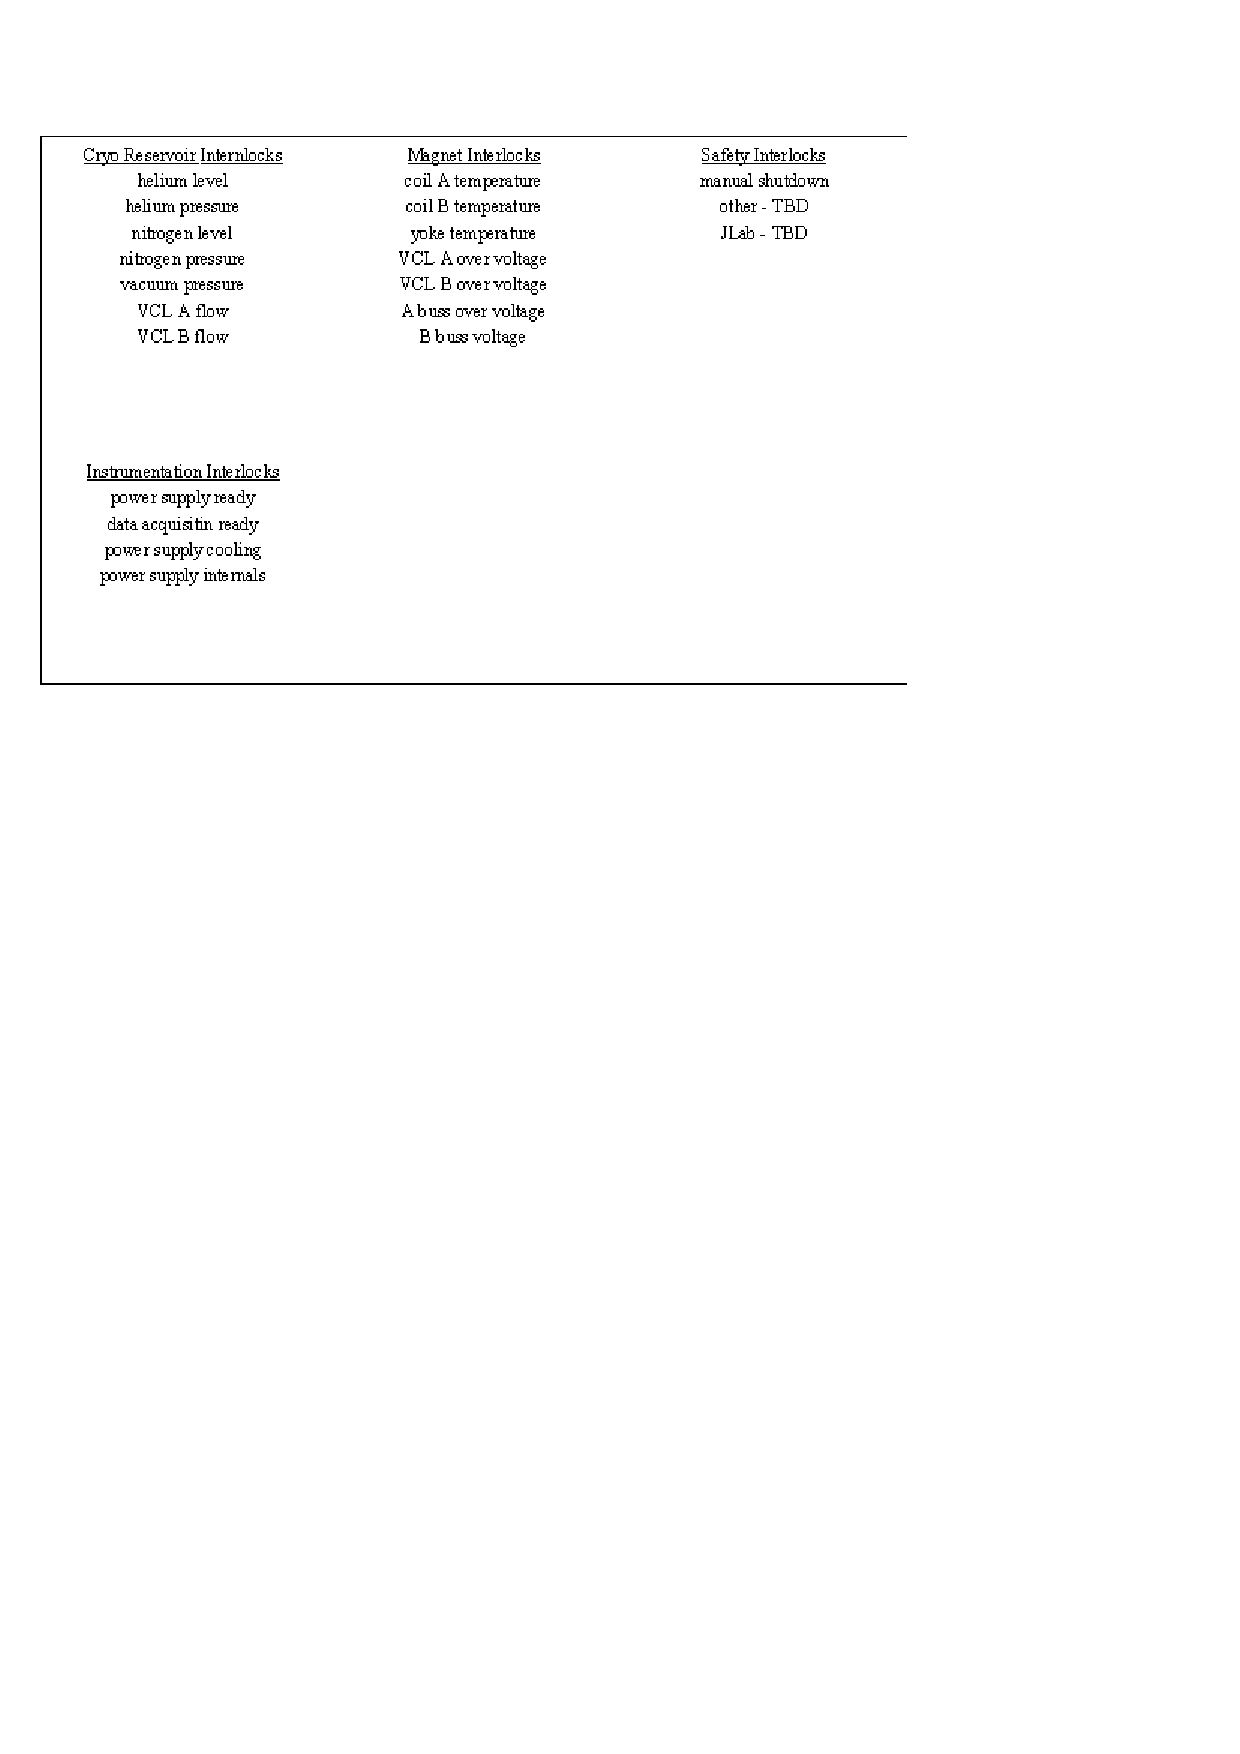
\includegraphics[angle=0,width=0.9\textwidth]{septum-interlocks}
\caption[Septum: Interlocks]{Septum magnet interlocks}  
\label{fig:septum-inter}
\end{center}
\end{figure}


Thresholds for the some of the conditions of the interlocks are set from the ``Setpoints" page which requires 
the Magnet Expert password.  All conditions are latched by the PLC.  Therefore, once a condition has faulted, 
the associated interlock will remain open, even if the condition is no longer in the fault state, until the 
reset button is pressed.  Each interlock chains is discussed in greater detail below.


{\bf The Slow Dump Interlock Chain:}
Any fault condition results in a slow dump (powered ramp-down) of the magnet power supply.  This happens 
in about 350 sec (6 min).


{\bf The Power Supply Interlock Chain:}
Conditions in this chain map directly to conditions maintained by the power-supply itself.  So this interlock 
chain is, in fact for display purposes.  The power supply is hardware interlocked by these conditions and will 
not go to the ON state unless are met. 


{\bf The Turn-On Interlock Chain:}
In addition to the hardware power supply interlocks, additional conditions must be met before the PLC permits 
the supply to be activated.  It is important to note that once the supply is acti-vated, a fault on the turn-on 
interlock chain does not necessarily cause the supply to turn off.  However, most of the turn-on interlock 
chain conditions also appear in one form or another on the slow or fast dump chains.


{\bf The Quench Interlock Chain:}
This chain is only satisfied if no coils have sensed a quench according to the digital quench pro-tection system.


{\bf The Fast Dump Interlock Chain:}
Any fault condition results in a fast dump of the magnet energy.  This happens in about 90s

\subsection {\bf Monitoring systems}

The monitoring of the SSMS is carried out by the user interface program running on the 
console PC.  This program, written using the LookoutDirect Human-Machine Interface (HMI) system, provides 
numeric and graphical information about all subsystems of the SEPTUMS SSMS.  A historical data base is 
maintained in compressed form on the local disk.  All parameters provided by the PLC are recorded to the 
data base.  The Lookout program also maintains an event log which includes information about ``button presses" 
and parameter adjustments made at the console.

An important function of the Lookout program is management of alarms, defined as events which require attention 
of the experiment shift staff or Magnet Expert.  Each alarm condition is identified by a number and all appear 
on the alarms control page.  Some alarms map directly into conditions incorporated in the interlock chains 
and so may cause the PLC to take some action, such as initiating a fast dump.  Alarming may be disabled for any 
of the alarm conditions (this does not prevent the PLC from taking action though).  If enabled to do so, the 
control system will phone a digital pager carried by the magnet on-call person and transmit the alarm number 
when an alarm occurs and is enabled.  In order to test the paging system, a special ``just checking in" alarm 
can be programmed to call the magnet on-call person periodically.

} %infolev

\infolevtwo{
\section{Operation of the HRS Magnets}

\subsection{Introduction}

This is an abbreviated operating manual for 
the HRS superconducting magnets specifically designed for Hall A 
experimenters.  It provides instructions for setting currents, invoking 
NMR field regulation and general system monitoring.  Curious readers are 
directed to the references for more in-depth operating instructions and 
other technical manuals. Copies of the following supporting
documents are available in the Hall A Control Room 
(see Table~\ref{tab:hrs-mag-manuals}).

\begin{table}[htp]
\begin{center}
\begin{tabular}{|l|l|}
\hline
References & \\
\hline 
WANG NMR Dipole & Operation Manual Power Supply \\
Dynapower & User Manual \\
Appendix & NMR Tesla meter \\
Appendix & NMR Field REgulation \\
Siemens/Fug & Q2/Q3 Power Supply Manual \\
Saclay/Danfusik & Q1 Powersupply Manual \\
TOSP & HRS Dipole \\
TOSP & HRS Quadrupole Q1 \\
TOSP & HRS Quadrupole Q2, Q3 \\
HRS & SC Dipole Magnet Safety Review Vol. 2 \\
HRS & SC Quad Safety Review Vol. 1 \\
OSP & HRS Septum Magnets \\ \hline
\end{tabular}
\end{center}
\caption[HRS Magnets: extra manuals]{HRS Magnets: extra manuals available in 
     Hall A Control Room.}
\label{tab:hrs-mag-manuals}
\end{table}

\subsection{Simple HRS Setting (Autopilot Mode)}
\label{sec:hrs-mag-set} 

 The magnets are controlled remotely using EPICS~\cite{EPICSwww} and
 MEDM~\cite{MEDMwww} GUI, provided that everything is working and power 
 supplies are turned on and ready to go.
 The appropriate interface runs
 on computer \mycomp{hacsbc2} (see Section \ref{sec:contr-ha-menu}).
 On the ``Hall A General Tools'' control screen, in the upper left, there is 
 a rectangular box for each spectrometer that (see Figure~\ref{fig:hrs_mag_cntrl}). 
\begin{figure}
\begin{center}
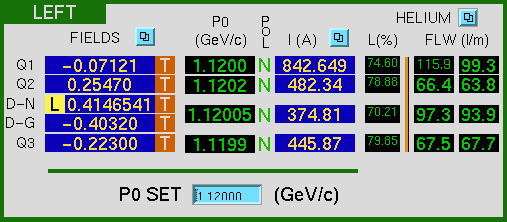
\includegraphics[angle=0,width=0.8\textwidth]{medm_halla_tools_1_cut1}
{\linespread{1.}
\caption[HRS: Magnets control]{A part of ``Hall A General Tools'' screen, 
        used for HRS (left) magnets control.}
\label{fig:hrs_mag_cntrl}}
\end{center}
\end{figure}

This box displays a brief summary of the status of the spectrometer
magnets and their cryogenic systems. The blue fields (with white
numbers) give readbacks of the magnetic fields and currents in each
magnet. The black fields also give readbacks, however in this case if
the text appears green those parameters are OK while if they are red
then that parameter is out of tolerance and may indicate a fault
condition. For example if the helium level goes below a certain point
the magnet will be automatically turned off.  In some cases it may be
desirable to monitor certain critical quantities on a strip chart
(e.g. Magnet settings). A strip chart tool is available for this
purpose from the bottom of the main control screen.

{\bf To set the spectrometers} for a given value of central momentum
(P0) type the desired P0 value into the yellow P0 SET box and hit
return. The magnets (except the septa magnets) will be automatically 
set to the correct
values. All green numbers in the P0 column indicates that the desired
field or current settings have been reached. 

Setting the septa magnets is described in Section \ref{sec:septum-start}. 

{\bf Caution:} Regarding the
dipoles, in general it's a bad idea to assume that at the first
instant that the P0 display turns green that the desired field has
been reached and you can start taking data. Stable field is in general
not achieved for from 15 to 30 minutes after reaching the nominal
desired field. This settling time depends on the magnet (Hadron is
slower than Electron) and the magnitude of the field change (small
changes settle faster than big changes). Experimenters are advised to
observe both the field reading and current reading on the magnet in
question and verify that things are stable to their satisfaction
before proceeding.
 
\subsection{Powering Up Dipole Magnets:}

Use these instructions to recover from loss of a magnet due to a fault
(e.g. He level or lead flow fault). The order of actions matters. \\
(Contact Tech on call if anything behaves funny or things don't
respond as expected. Sometimes after a trip an access to the Hall is
required to reset things).

\begin{list}{\arabic{enumi}.~}{\usecounter{enumi}\setlength{\itemsep}{-0.15cm}}
   \item Wait for Iout=0 (you can't and don't want to do anything while the magnet is in emergency fast dump mode.)
   \item While waiting, make a log entry re the fault. Give details such as time, coincident activities, and nature of the fault.
   \item Make sure the fault is cleared. (e.g. He level and flow rates returned to normal values and stable)
   \item In the HRS Hadron (Electron) Dipole Systems' control panel:
   \begin{list}{}{\setlength{\itemsep}{-0.15cm}}
      \item[(a)] Press RESET (verify that all faults are cleared in the middle column)
      \item[(b)] Press START (Display will indicate Power Supply ON and magnet ENGAGED)
   \end{list}
\end{list}


Power supply and magnet are ready to go. From here you can return 
to "Autopilot Mode" (see Section \ref{sec:hrs-mag-set}).

\subsection{Starting Q1 Power Supply:}

 Do this when a fault causes the power supply to shut off.
 Wait for fault to clear (watch He levels). 
\begin{list}{\arabic{enumi}.~}{\usecounter{enumi}\setlength{\itemsep}{-0.15cm}}
   \item Push RESET (check all faults cleared)
   \item Select desired polarity
   \item Push ON
   \item Type in ISET (yellow field) or re-enter P0 in Autopilot Mode.
\end{list}

\subsection{Starting Q2/3 Power Supply:}

 Do this when a fault causes the power supply to shut off.
 Wait for cause of fault to clear (watch He levels). 
 \begin{list}{\arabic{enumi}.~}{\usecounter{enumi}\setlength{\itemsep}{-0.15cm}}
   \item Push RESET 
   \item Select desired polarity
   \item Push ON
   \item Type in ISET (yellow field) or re-enter P0 in Autopilot Mode.
\end{list}

\subsection{Starting a Septum Magnet}
\label{sec:septum-start}

The EPICS screen for septum magnet control can be accessed as follows. From the Hall A Main Menu select
 Magnet Controls then from the activated pull down menu select Septum Right 0r Left Controls. A copy of
 the EPICS screen is shown in Figure~\ref{fig:septum_cntrl} .

\begin{figure}
\begin{center}
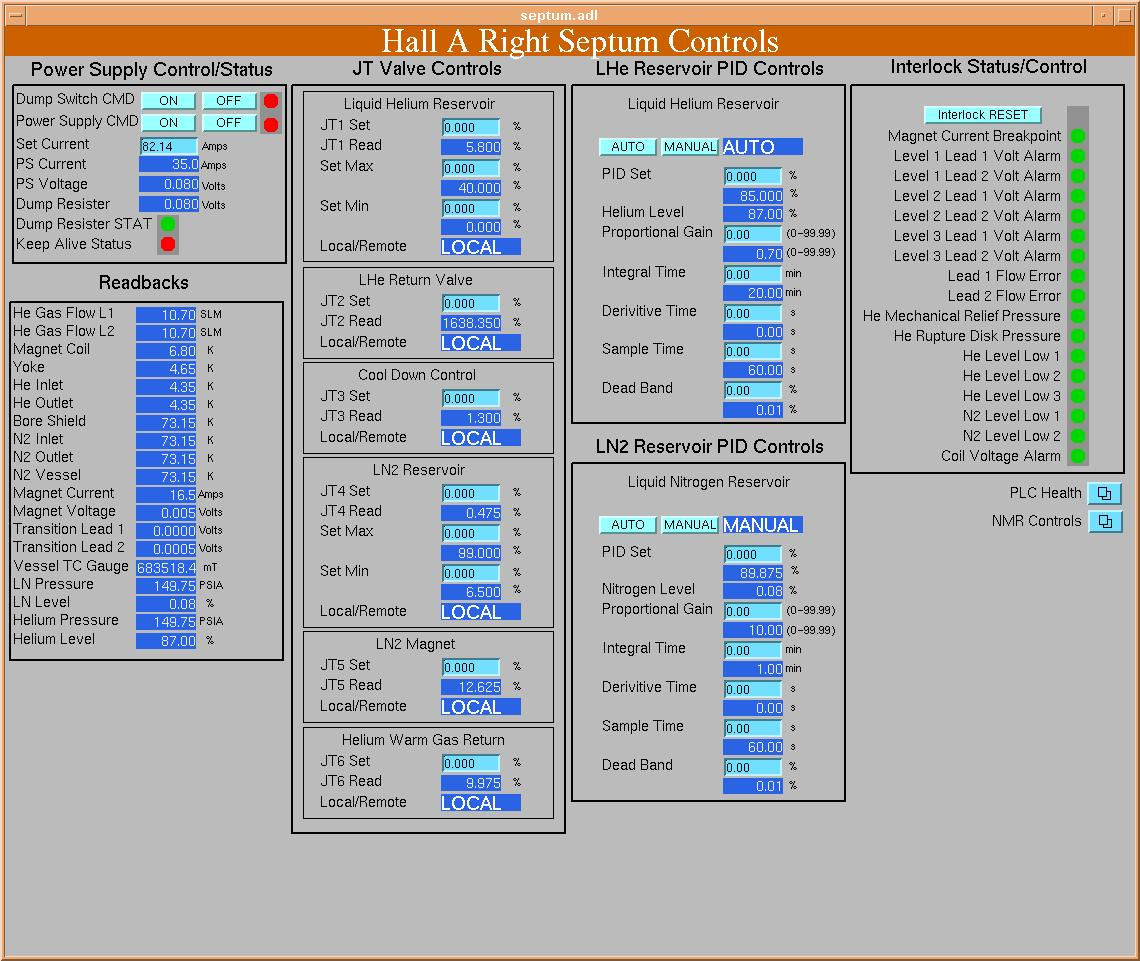
\includegraphics[angle=0,width=0.9\textwidth]{septum_control}
{\linespread{1.}
\caption[Spectrometers:Septum Controls Screen]{Septum Controls Screen.}
\label{fig:septum_cntrl}}
\end{center}
\end{figure}
 
Please note that the cycle from command to action can be quite slow so
expect to wait many seconds for an indication of command
execution. While it is more usual to use the HRS spectrometer Momentum
setting routine to set all the HRS magnets including the septum the
septum can also be run standalone. The steps below must be used to
prepare septum for energization in either case.

\noindent Energizing the septum:\\

\noindent {\bf n.b.} Except for step 1, which requires a Hall access,
NEVER proceed to the next step without successfully completing the
verifying observation. If the verifying observation is not satisfied
call an expert for consultation.

\begin{list}{\arabic{enumi}.~}{\usecounter{enumi}\setlength{\itemsep}{-0.15cm}}
  \item Turn on Power supply in the Hall\\  
  \item Clear interlocks and observe all green status in upper
      right of Septum Controls page
  \item Verify operating conditions. Observe: Coil Temperature =
      7 K, Helium Level $\ge85\%$ , He Gas Flow L1 and L2 about 10.6 SLM
  \item Dump Switch CMD ON then observe green light next to ON/OFF
 
  \item Power Supply CMD ON then Observe green light next to ON/OFF
  \item Enter p0 in the po set box as with other magnets or enter
   desired current in the Set Current box then observe magnet coil
   voltage and current increase
  \item Continuously verify proper operation. He Gas Flow L1 and
     L2 should increase with current.  Coil temperature drops during
     ramping. A slight initial increase at start of ramp is normal.  The
     coil Temperature drops significantly at 100 Amps and reaches ~ 6.3 K
     at 350 Amps
\end{list}
 
 
} %infolev

\infolevthree{
\vspace*{0.5in}
\begin{table}[hp]
\begin{tabular}{ll}
\\
Circuit Parameters: & \\
Imax = 1800 A, L = 2.52H, Tau(slow) = 420 s, 640 MITS & \\
Rdish = dump resistor + cable resistance = total resistance & \\
Rtotal = .0045 + .0015 = .006 $\Omega$ & \\
Rdump .134 $\Omega$ , L= 2.55 H, Tau(fast) = 19 s, 29 MITS & \\
Magnet Dipole & signature, date \\
Arm (Circle one)-Electron Arm, Hadron Arm & \underline{\hskip1in}\\
Megger check of coil @ 250 V DC\underline{\hskip0.5in} & 
\underline{\hskip1in}\\
Visual inspection walk through & \underline{\hskip1in}\\
Set water inlet pressure to 100 psi\underline{\hskip0.5in} & 
\underline{\hskip1in} \\
Coil A Trip Voltage (1.2V+) value \underline{\hskip0.5in} & 
\underline{\hskip1in}\\
Coil B Trip Voltage (1.2V-) value \underline{\hskip0.5in} & 
\underline{\hskip1in}\\
*Magnet Lead A Trip (1.2V+) \underline{\hskip0.5in} & 
\underline{\hskip1in}\\
*Magnet Lead B Trip (70mV) value \underline{\hskip0.5in} & 
\underline{\hskip1in}\\
*Magnet Leads are not bipolar and only work in the PS forward 
polarity.\\
Magnet lead A must be connected to the PS+ & \\
Level Trip (70\%) value \underline{\hskip0.5in} & 
\underline{\hskip1in}\\
Magnet Flow A Trip (60 SLPM) value \underline{\hskip0.5in} & 
\underline{\hskip1in}\\
Magnet Flow B Trip (60 SLPM) value \underline{\hskip0.5in} & 
\underline{\hskip1in}\\
Operational Test of trips \underline{\hskip0.5in} & 
\underline{\hskip1in}\\
PS overcurrent trip (2000A) \underline{\hskip0.5in} & 
\underline{\hskip1in}\\
See manual for voltage setting and gain (4V=800A) & \\
Magnet Ready for Operation & \underline{\hskip1in} 
\end{tabular}
\caption[Spectrometers: Dipole Checklist]{Hall A Dipole Magnet Check List (15 August 1996) }
\label{tab:dip_check}
\end{table}


\begin{table}[hp]
\begin{tabular}{ll}
Circuit Parameters: & \\
Rext = 0.075 $\Omega$, L = 25 mH, Tau = 0.3 s, Vthreshold = .1V Imax
= 3250A \\
Magnet (Circle one) - Q1, & \underline{\hskip1in} \\
Arm (Circle one) - Electron Arm, Hadron Arm & \underline{\hskip1in} \\
Visual inspection walk through & \underline{\hskip1in} \\
Set water pressure at 100 psi inlet \underline{\hskip0.5in} & 
\underline{\hskip1in} \\
Coil A Trip Voltage {+} value\_25mV \underline{\hskip0.5in} & 
\underline{\hskip1in} \\
Coil B Trip Voltage (-) value\_25 mV \underline{\hskip0.5in} & 
\underline{\hskip1in} \\
Magnet Lead A Trip (+) Voltage\_80 mV \underline{\hskip0.5in} & 
\underline{\hskip1in} \\
Magnet Lead B Trip (-) Voltage\_80 mV \underline{\hskip0.5in} & 
\underline{\hskip1in} \\
Level Trip percent 980\%  \underline{\hskip0.5in} & 
\underline{\hskip1in} \\
Magnet Flow A Trip (30 SLPM+) setting \underline{\hskip0.5in} & 
\underline{\hskip1in} \\
Magnet Flow B Trip (30 SLPM-) setting \underline{\hskip0.5in} & 
\underline{\hskip1in} \\
Operational test of trips \underline{\hskip0.5in} & 
\underline{\hskip1in} \\
Magnet Ready for Operation & \underline{\hskip1in} \\
{} & \underline{\hskip1in} 
\end{tabular}
\caption[Spectrometers: Q1 Checklist]{Hall A Q1 Quadrupole Magnet Check List (15 August 1996)} 
\label{tab:q1_check}
\end{table}

\begin{table}[hp]
\begin{tabular}{ll}
Circuit Parameters: & \\
Rext = .125 $\Omega$, Tau = 3 s, Quench Vthreshold = .1V, Imax = 1850A \\
Magnet (Circle one) - Q2, Q3 & \underline{\hskip1in} \\
Arm (Circle one)-Electron Arm, Hadron Arm & \underline{\hskip1in} \\
Visual inspection walk through & \underline{\hskip1in} \\
Meggelr Magnet @ 250 V DC \underline{\hskip0.5in} & 
\underline{\hskip1in} \\
Set water pressure at 100 psi inlet \underline{\hskip0.5in} & 
\underline{\hskip1in} \\
Coil A Trip Voltage (+) value \underline{\hskip0.5in} & 
\underline{\hskip1in} \\
Coil B Trip Voltage (-) value \underline{\hskip0.5in} & 
\underline{\hskip1in} \\
Magnet Lead A Trip (+) Voltage \underline{\hskip0.5in} & 
\underline{\hskip1in} \\
Magnet Lead B Trip (-) Voltage \underline{\hskip0.5in} & 
\underline{\hskip1in} \\
Magnet Lead Trip (trim) Voltage \underline{\hskip0.5in} & 
\underline{\hskip1in} \\
Level Trip percent (80\%) \underline{\hskip0.5in} & 
\underline{\hskip1in} \\
Magnet Flow A Trip (50 SLPM+) setting \underline{\hskip0.5in} & 
\underline{\hskip1in} \\
Magnet Flow B Trip (50 SLPM-) setting \underline{\hskip0.5in} & 
\underline{\hskip1in} \\
Magnet Flow trim Trip (3.6 SLPM) setting \underline{\hskip0.5in} & 
\underline{\hskip1in} \\
Operational test of trips \underline{\hskip0.5in} & 
\underline{\hskip1in} \\
Magnet Ready for Operation \underline{\hskip0.5in} & 
\underline{\hskip1in} \\
& \underline{\hskip1in}
\end{tabular}
\caption[Spectrometers: Q2/Q3 Checklist]{Hall A Q2/Q3 Quadrupole Magnet Check List  (15 August 1996)}
\label{tab:q23_check}
\end{table}

} %infolev

